\section{Exact multivariate amplitude distributions}
\label{sec:exact_distributions}

% In Sect. \ref{subsec:time_definition} we describe the physical time scale and
% the trade time scale. In Sect. \ref{subsec:trade_time} and Sect.
% \ref{subsec:physical_time} we define the trade and the physical time scales,
% respectively.

%%%%%%%%%%%%%%%%%%%%%%%%%%%%%%%%%%%%%%%%%%%%%%%%%%%%%%%%%%%%%%%%%%%%%%%%%%%%%%%
\subsection{Key concepts}\label{subsec:key_concepts}

Consider time series $S_{k} \left( t \right)$, $k = 1, 2, \ldots, K$ of stock
prices for $K$ companies. The values $S_{k} \left( t \right)$ are taken in
fixed time steps $\Delta t$. In general, the data contain an exponential
increase due to the drift. Thus, to measure the correlations independently of
this trend, it is better to use logarithmic differences instead of returns
\begin{equation}
    G_{k} \left( t \right) = \ln S_{k} \left( t + \Delta t \right) -
    \ln S_{k} \left(t \right) = \ln \frac{S_{k} \left( t + \Delta t \right)}
    {S_{k} \left(t \right)}.
\end{equation}
Anyway, logarithmic differences and returns almost coincide if the time steps
$\Delta t$ are sufficiently short \cite{subtle_nature,empirical_facts}
\begin{equation}
    G_{k} \left(t\right) \approx r_{k} \left(t\right)
    = \frac{S_{k} \left( t + \Delta t \right) - S_{k} \left( t \right)}
    {S_{k} \left( t \right)}.
\end{equation}
The returns are well known to have distributions with heavy tails, the smaller
$\Delta t$, the heavier
\cite{non_stationarity_fin_guhr}. Furthermore, the sample standard deviations
$\sigma_{k}$, referred to as volatilities, strongly fluctuate for different
time windows of the same length $T$
\cite{non_stationarity_fin_guhr,volatility_change}.

The mean of the logarithmic differences reads \cite{exact_distributions_guhr}
\begin{equation}
    \left\langle G_{k} \left( t \right) \right\rangle_{T} = \frac{1}{T}
    \sum_{t = 1}^{T} G_{k} \left( t \right).
\end{equation}
To compare the different $K$ companies, it is necessary to normalize the time
series. The normalized time series are defined by
\cite{exact_distributions_guhr,non_stationarity_fin_guhr}
\begin{equation}
    M_{k} \left( t \right) = \frac{G_{k} \left( t \right) - \left\langle
    G_{k} \left( t \right) \right\rangle} {\sqrt{\left\langle G_{k}^{2}
    \left( t \right) \right\rangle_{T} - \left\langle G_{k} \left( t \right)
    \right\rangle^2_{T}}},
\end{equation}
where
\begin{equation}
    \sigma_{k} = \sqrt{\left\langle G_{k}^{2}
    \left( t \right) \right\rangle_{T} - \left\langle G_{k} \left( t \right)
    \right\rangle^2_{T}}
\end{equation}
is the volatility of the $k$ company in the time window of length $T$. These
values can be viewed as the elements of a $K \times T$ rectangular matrix $M$.
With these normalizations and rescalings, it can be measured correlations in
such a way that all companies and all stocks are treated on equal footing.

The correlation coefficient for the stocks $k$ and $l$ is defined as
\cite{non_stationarity_fin_guhr}
\begin{equation}
    C_{kl} = \left\langle M_{k} \left( t \right) M_{l} \left( t \right)
    \right\rangle_{T} = \frac{1}{T} \sum_{t=1}^{T} M_{k} \left( t \right) M_{l}
    \left( t \right),
\end{equation}
which can be written as
\begin{equation}
    C_{kl} = \frac{\left\langle G_{k} \left( t \right) G_{l} \left( t \right)
    \right\rangle_{T} - \left\langle G_{k} \left( t \right) \right\rangle_{T}
    \left\langle G_{l} \left( t \right) \right\rangle_{T}}
    {\sigma_{k} \sigma_{l}}.
\end{equation}
The coefficients $C_{kl}$ are the elements of a $K \times K$ square matrix $C$,
the correlation matrix. The limiting values of these correlation coefficients
\begin{equation}
    C_{kl}^{\text{lim}} =
    \left\{
    \begin{array}{cc}
    +1 & \text{completely correlated}  \\
    0  & \text{completely uncorrelated}\\
    -1 & \text{completely anticorrelated}
    \end{array}
    \right. .
\end{equation}
The time average of $C_{kl}$ can be viewed as the matrix product of the
rectangular matrix $M$ ($K \times T$) with its transpose matrix $M^{\dagger}$
($T \times K$), divided by $T$. Thus, the correlation matrix can be written in
the form
\begin{equation}
    C = \frac{1}{T} M M^{\dagger}.
\end{equation}
The correlation matrix $C$ is real and symmetric. Using the correlation matrix
$C$ is possible to define the covariance matrix
\cite{credit_risk_guhr,portfolio_distributions_guhr,asset_correlations_guhr,stochastic_cov_guhr,exact_distributions_guhr}
\begin{equation}
    \Sigma = \sigma C \sigma ,
\end{equation}
where the diagonal matrix $\sigma$ contains the volatilities $\sigma_{k}$,
$k = 1, \ldots, K$.

From the results obtained in
\cite{portfolio_distributions_guhr,non_stationarity_fin_guhr}, it does not make
a difference the calculation with a covariance or a correlation matrix. Thus,
to ease the comparison between works, we will use covariance matrices as in
\cite{non_stationarity_fin_guhr}.

\begin{figure}[htbp]
    \centering
    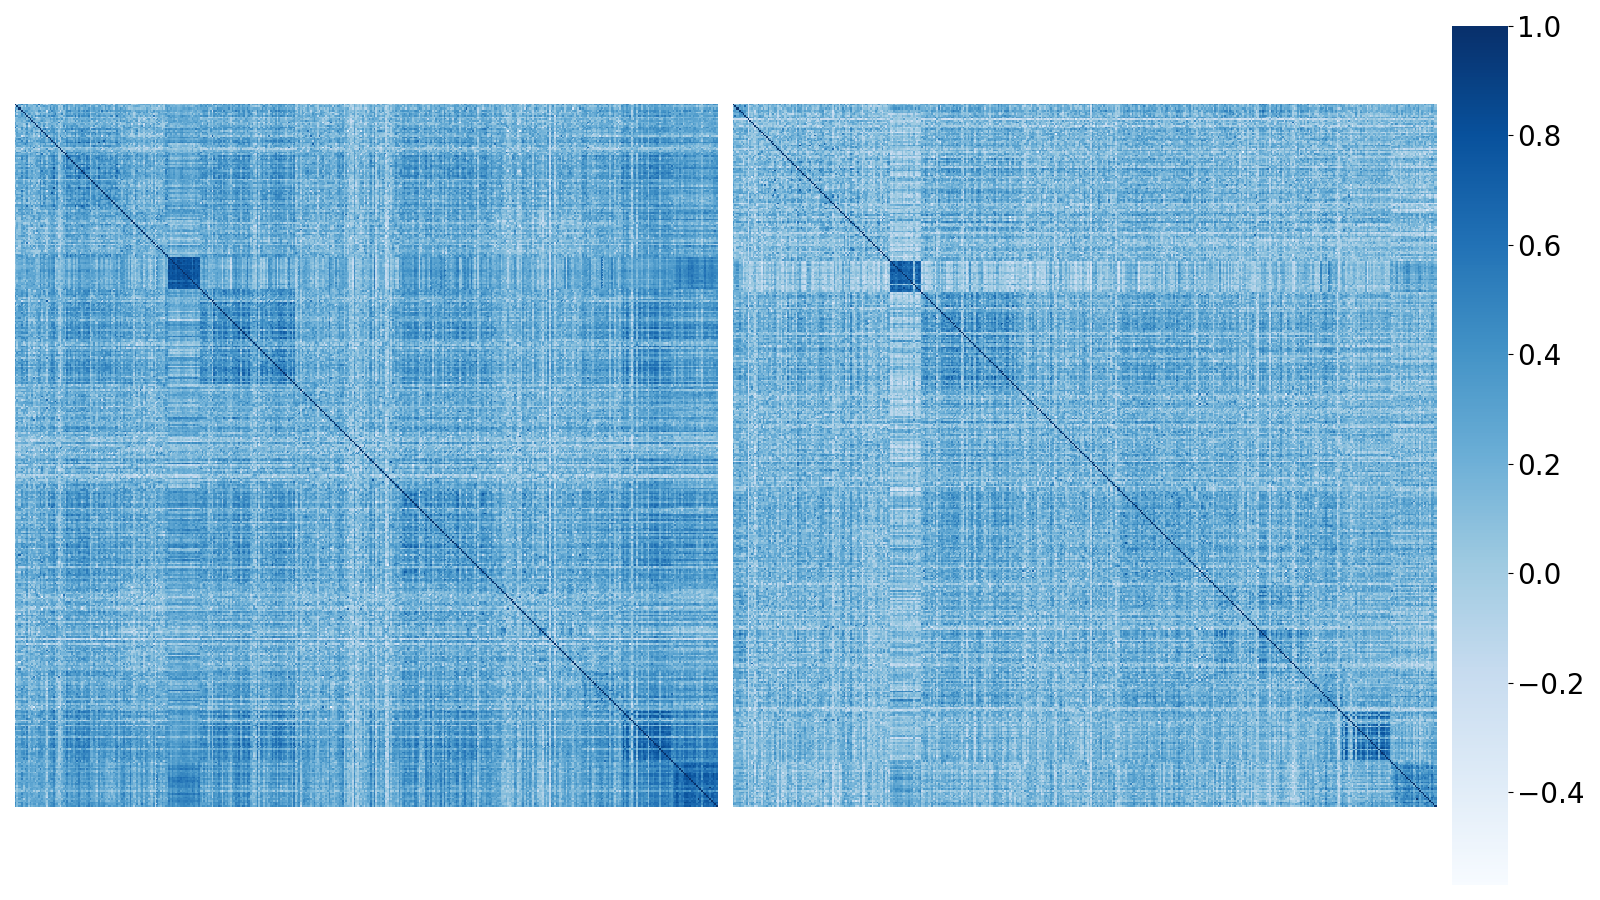
\includegraphics[width=\columnwidth]
    {figures/03_correlation_matrix.png}
    \caption{Correlation matrices of $K = 421$ companies for the fourth quarter
             of 2005 (left) and the first quarter of 2006 (right), the darker,
             the stronger the correlation. The companies are sorted according
             to industrial sectors.}
    \label{fig:correlation_matrices}
\end{figure}


%%%%%%%%%%%%%%%%%%%%%%%%%%%%%%%%%%%%%%%%%%%%%%%%%%%%%%%%%%%%%%%%%%%%%%%%%%%%%%%
\subsection{General considerations}\label{subsec:general_considerations}

To compare the $K$ variate distributions with data, the crucial idea is to
construct $K$ univariate distributions out of the $K$ variate one which are
then overlaid \cite{exact_distributions_guhr}. To decouple the amplitudes, we
rotate the vector $r$ into the eigenbasis of the correlation matrix C or the
eigenbasis of the covariance matrix $\Sigma$
\cite{non_stationarity_fin_guhr,exact_distributions_guhr}. More precisely, we
use the diagonalization
\begin{align}
    C = U \Lambda U^{\dagger} \text{ such that }
    C^{-1/2} = U \Lambda^{-1/2} U^{\dagger}
\end{align}
or
\begin{align}
    \Sigma = U \Lambda U^{\dagger} \text{ such that }
    \Sigma^{-1/2} = U \Lambda^{-1/2} U^{\dagger},
\end{align}
where $U$ is an orthogonal $K \times K$ matrix and $\Lambda$ is the diagonal
matrix of the eigenvalues $\Lambda_{k}$. As they are positive definite, the
square roots $\Lambda_{k}^{1/2}$ are real, we choose them positive. We use the
rotated amplitudes
\begin{equation}
    \tilde{r} = U^{\dagger} r
\end{equation}
as new arguments of the ensemble averaged amplitude distribution.

When analyzing data, $K$ is given, we obtain the matrices $C$ and $\Sigma$ by
using the originally measured amplitudes for sampling over the long time interval.
In all cases, the parameter N is a fit parameter, measuring the strenght of the
fluctuations. Experience tells, that $N$ sensitevily determines the shape and is
best obtained by fitting the whole distribution to the data.

%%%%%%%%%%%%%%%%%%%%%%%%%%%%%%%%%%%%%%%%%%%%%%%%%%%%%%%%%%%%%%%%%%%%%%%%%%%%%%%
\subsection{Four cases distributions}\label{subsec:distributions}

In the Gaussian-Gaussian case with the Markovian situation $D = \mathbb{1}_{N}$
the distribution reads
\begin{equation}
    \begin{split}
    \left\langle p \right\rangle_{GG}^{\left(k\right)}
    \left(\tilde{r}_{k} \vert \Lambda_{k}, \mathbb{1}_{N}\right) &=
    \frac{1}{2^{\left(N - 1\right) / 2} \Gamma \left(N / 2\right)
    \sqrt{\pi \Lambda_{k} / N}} \\
    & \sqrt{\frac{N \tilde{r}_{k}^2}{\Lambda_{k}}}^{\left(N - 1\right) / 2}
    \operatorname{K}_{\left(1 - N\right)/2}
    \left( \sqrt{\frac{N \tilde{r}^2_{k}}{\Lambda_{k}}}\right),
    \end{split}
\end{equation}
In the Gaussian-algebraic case with the Markovian situation
$D = \mathbb{1}_{N}$ the distribution reads
\begin{equation}
    \begin{split}
    \left\langle p \right\rangle_{GA}^{\left(k\right)} &
    \left(\tilde{r}_{k} \vert \Lambda_{k}, \mathbb{1}_{N}\right) = \\
    &\frac{\Gamma\left(L - \left(K + N \right) / 2 + 1\right)
    \Gamma\left(L - \left(K - 1\right) / 2\right)}
    {\Gamma\left(L - \left(K + N - 1\right) / 2\right) \Gamma\left(N / 2\right)
    \sqrt{2\pi \Lambda_{k}M/N}} \\
    & \operatorname{U} \left(L - \frac{K + N}{2} + 1, \frac{1 - N}{2} + 1,
    \frac{N}{2M} \frac{\tilde{r}^{2}_{k}}{\Lambda_{k}}\right)
    \end{split}
\end{equation}
In the algebraic-Gaussian case with the Markovian situation
$D = \mathbb{1}_{N}$ the distribution reads
\begin{equation}
    \begin{split}
    \left\langle p \right\rangle_{AG}^{\left(k\right)} &
    \left(\tilde{r}_{k} \vert \Lambda_{k}, \mathbb{1}_{N}\right) = \\
    &\frac{\Gamma\left(l - \left(K - 1 \right) / 2\right)
    \Gamma\left(l - \left(K - N\right) / 2\right)}
    {\Gamma\left(l - K / 2\right) \Gamma\left(N / 2\right)
    \sqrt{2\pi \Lambda_{k}m/N}} \\
    & \operatorname{U} \left(l - \frac{K - 1}{2}, \frac{1 - N}{2} + 1,
    \frac{N}{2m} \frac{\tilde{r}^{2}_{k}}{\Lambda_{k}}\right)
    \end{split}
\end{equation}
Finally, in the algebraic-algebraic case with the Markovian situation
$D = \mathbb{1}_{N}$ the distribution reads
\begin{equation}
    \begin{split}
    \left\langle p \right\rangle_{AA}^{\left(k\right)} &
    \left(\tilde{r}_{k} \vert \Lambda_{k}, \mathbb{1}_{N}\right) = \\
    &\frac{\Gamma\left(l - \left(K - 1 \right) / 2\right)
    \Gamma\left(l - \left(K - N\right) / 2\right)}
    {\Gamma\left(l - K/ 2\right) \Gamma\left(L + l - \left(K - 1\right) \right)
    \sqrt{\pi \Lambda_{k}Mm/N}} \\
    &\frac{\Gamma\left(L - \left(K + N \right) / 2 + 1\right)
    \Gamma\left(L - \left(K - 1\right) / 2\right)}
    {\Gamma\left(L - \left(K + N - 1\right) / 2\right) \Gamma\left(N / 2\right)
    } \\
    & _{2}\operatorname{F}_{1} \left(l - \frac{K - 1}{2}, L -\frac{K + N}{2}+1,
    L + l - \left(K - 1\right), 1 - \frac{N}{Mm} \frac{\tilde{r}^{2}_{k}}
    {\Lambda_{k}}\right)
    \end{split}
\end{equation}

For a visual comparison of the distributions, we plot the GG, GA, AG and AA
distributions in the Markovian case in the same figure. In Fig. \ref{fig:distributions_comparison}
we consider $K = 100$ positions with shape parameters $L = 55$, $l = 55$, as
well as $N = 5$ which is a typical value from an empirical viewpoint. In the top
are the probability densities in linear scale and in the bottom are the probability
densities in logarithmic scales. From figure, it can be seen the more algebraic,
the stronger peaked is the distribution and heavier are the tails.

\begin{figure}[htbp]
    \centering
    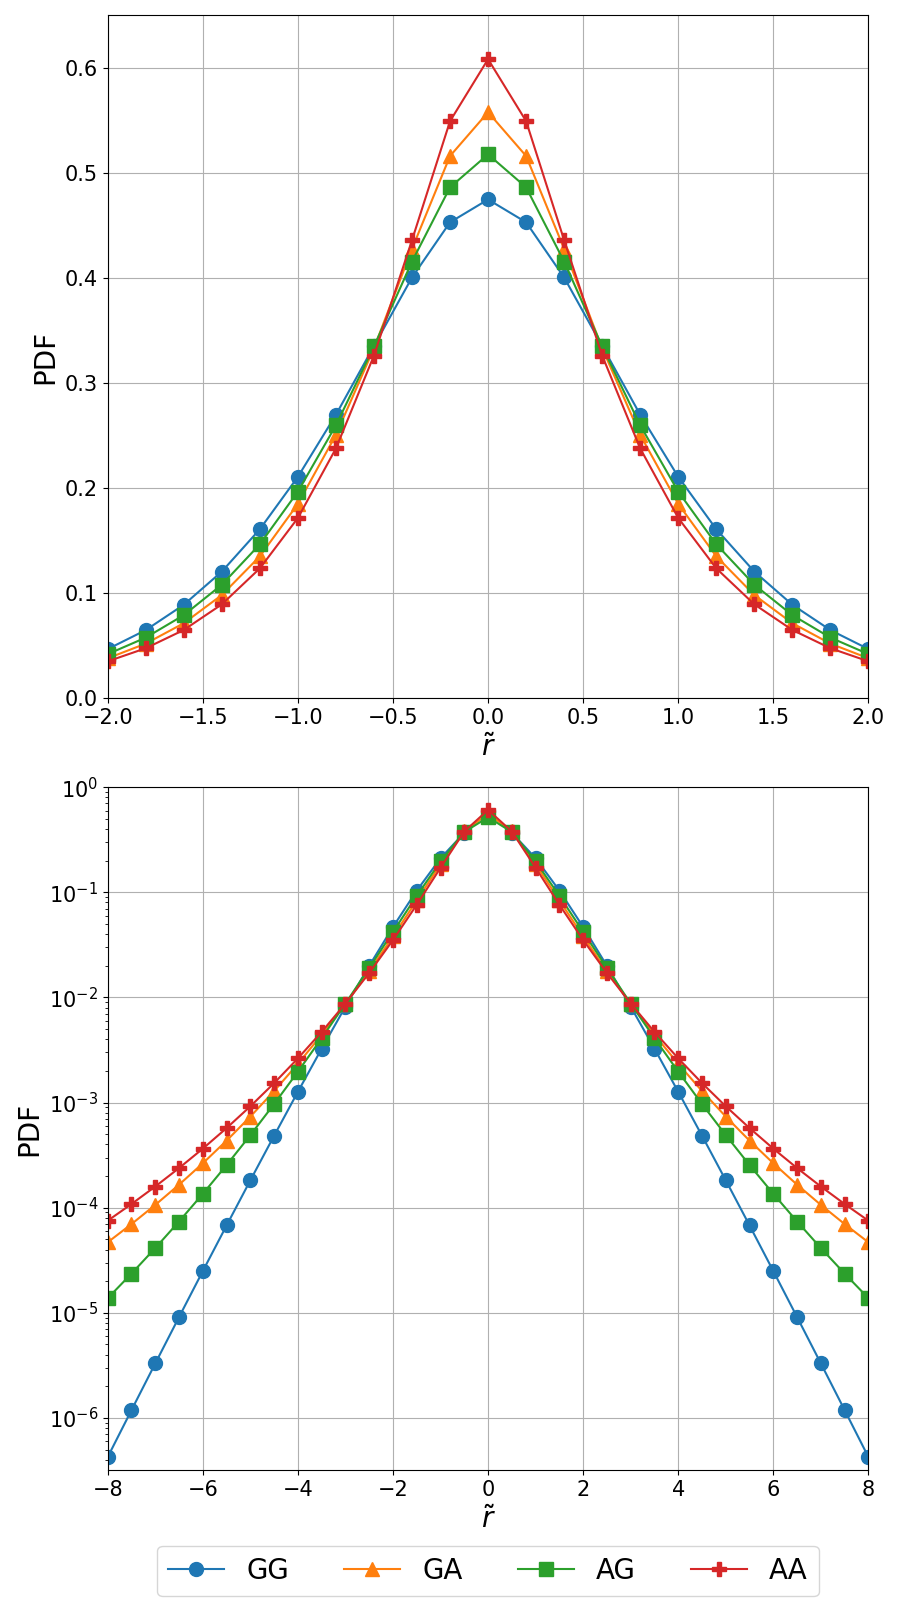
\includegraphics[width=\columnwidth]
    {figures/05_distributions_comparison.png}
    \caption{Probability densities $\left\langle p \right\rangle_{YY'}^{\left(k\right)}$,
             in the Markovian case versus the rotated amplitudes $\tilde{r}$,
             normalized to unit standard deviation. The four cases Gaussian-Gaussian,
             Gaussian-Algebraic, Algebraic-Gaussian and Algebraic-Algebraic are
             labeled $YY' = GG$, $GA$, $AG$ and $AA$, respectively. Number of
             positions $K = 100$, shape parameters $L = 55$ and $l = 55$, strength
             parameter for fluctuations of correlations $N = 5$. (Top) Linear scale,
             abscissa between $-2$ and $+2$ and (bottom) logarithmic scale, abscissa
             between $-8$ and $+8$.}
    \label{fig:distributions_comparison}
\end{figure}

%%%%%%%%%%%%%%%%%%%%%%%%%%%%%%%%%%%%%%%%%%%%%%%%%%%%%%%%%%%%%%%%%%%%%%%%%%%%%%%
\subsection{Graphical representations}\label{subsec:graphical_distributions}

To plot a comparison of the distributions involving algebraic distributions
with those in the Gaussian-Gaussian case, we choose values of $L$ and $l$ which
ensure the existence of the first matrix moment (?). We notice that the
conditions on the existence of the algebraic distributions, i.e., of their
normalizations, are slightly weaker. The variances $\left\langle \tilde{r}_{k} \right\rangle_{YY'}{\left(k\right)}$
are simply given by $\Lambda_{k}$. The functional form of all distributions
$\left\langle p \right\rangle_{YY'}{\left(k\right)} \left(\tilde{r}_{k} \vert D \right)$
then allows us to normalize the rotated amplitude $\tilde{r}_k$ by the standard
deviation

\begin{equation}
    \tilde{r} = \frac{\tilde{r}_{k}}{\sqrt{\Lambda_{k}}}
\end{equation}

such that all $K$ distributions in this variable coincide and the corresponding
variances are all given by one.